\section{Conclusion}

I started working on this system on 1st of October and the development ended on 12nd of November, for a global amount of 240 hours of workload.
I'd like to highlight the main difficulties I found and how I fixed them, but it's something I'm going to do during the presentation of the project.
\newline
Approximately, considering all hardware I bought, not what I burnt, this kind of system costs 150 euros. Anyway, that price will be lower for sure. If I wanted to draw a real circuit PCB, for sure I would use the embedded ADC of the microcontroller; moreover I would choose a microcontroller having a smaller number of pins, so removing a lot of peripherals that I didn't initialize; then, the implementation by PCB would make the breadboard useless.
\newline
Another thing that I could improve is the Python script to re-build images. Currently it just generates black and white pictures, a better code would fill them by colors.
\newline
A further step consists in resizing components in Buck circuit, in order to optimize consumptions. Some other pictures follow and end the report.
\begin{figure}[H]
\centering
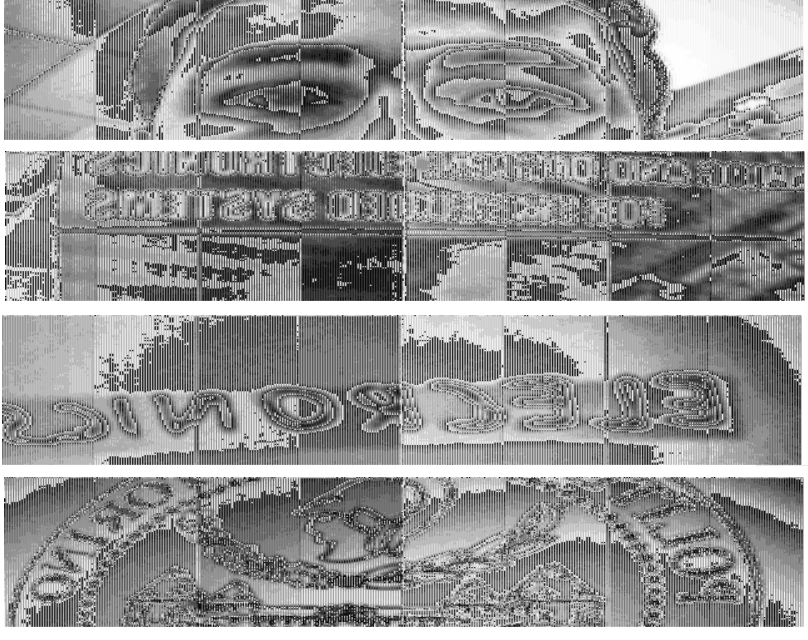
\includegraphics[scale=.9]{Immagini/test99}
\label{04}
\end{figure}

